% TODO Label the regions in the saturation graph
\FloatBarrier

\begin{figure}[h!]
	\centering
	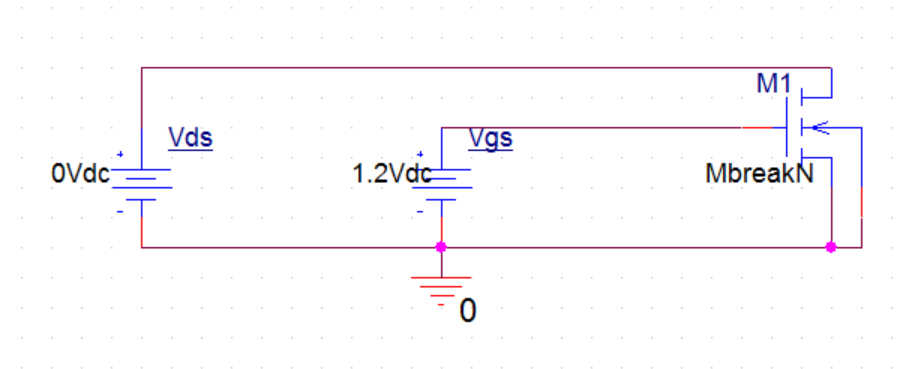
\includegraphics[scale=0.5]{./images/circuit1.PNG}
	\caption{NMOS Circuit}
	\label{fig:circuit1}
\end{figure}

\FloatBarrier

In general, NMOS transistors have three operation modes. The first mode is cutoff, where $V_{GS} < V_{T}$, where $V_{T}$ is the threshold voltage. The NMOS structure uses a MOS capacitor in the middle. Below the threshold voltage, not enough minority carriers exist in the bulk's conduction band to actually drive a substantial current. In the case of an NMOS transistor, the bulk is p-type, meaning minority carriers are electrons. Thus, when $V_{GS} < V_{T}$ in the NMOS, the drain current due to the minority carrier electrons is effectively $0$\si{\milli\ampere}. \\

By setting a voltage at the gate, the majority carrier holes in the p-type substrate are pushed away, exposing the negative acceptor ions beneath them. A depletion region forms as a result. Once the gate voltage exceeds the threshold voltage, valence band electrons in the depletion region acquire enough energy to jump the bandgap and become conduction electrons. As a result, an inversion layer develops in the bulk between the source and the drain. A drain current can now flow. \\

When $V_{GS} > V_{T}$, a bifurcation occurs. The NMOS can either enter the triode or saturation mode. In the triode mode, the NMOS acts as an approximately linear resistor. The conductivity, and therefore the resistance, can be controlled by varying the number of minority carrier electrons by changing the gate voltage. By applying $V_{DS}$, a current is then driven through the somewhat linear resistance. For small values of $V_{DS}$, the resistance is basically linear. For larger values, the resistance begins to act less linear, but still exhibits similar behavior. The MOSFET remains in this triode mode for as long as $V_{DS} < V_{GS} - V_{T}$. However, once $V_{DS} > V_{GS} - V_{T}$, the MOSFET enters saturation. In the saturation mode, the NMOS does not have enough carrier electrons in the channel to support the desired current that should be present given $V_{DS}$. At this point, increasing $V_{DS}$ leads to no additional current past the saturation current.

However, in the saturation mode, as $V_{DS}$ is increased, more electrons concentrate toward the source than the drain. At saturation, no excess carrier electrons exist at the drain, and the channel "pinches-off" as a result. Past this point, the channel length decreases because more and more of the area closer to the drain becomes unoccupied by electrons as they move toward the source. As the channel becomes shorter, its resistance decreases, and the current increases linearly. This effect is known as channel length modulation. So, the saturation current looks like:

\begin{equation}
	\label{eq:sat_current_clm}
	i_D = \frac{k_n}{2} ( V_{GS} - V_{T} )^2 ( 1 + \lambda V_{DS} ) \ ( \lambda: constant )
\end{equation}

\FloatBarrier

\begin{figure}[h!]
	\centering
	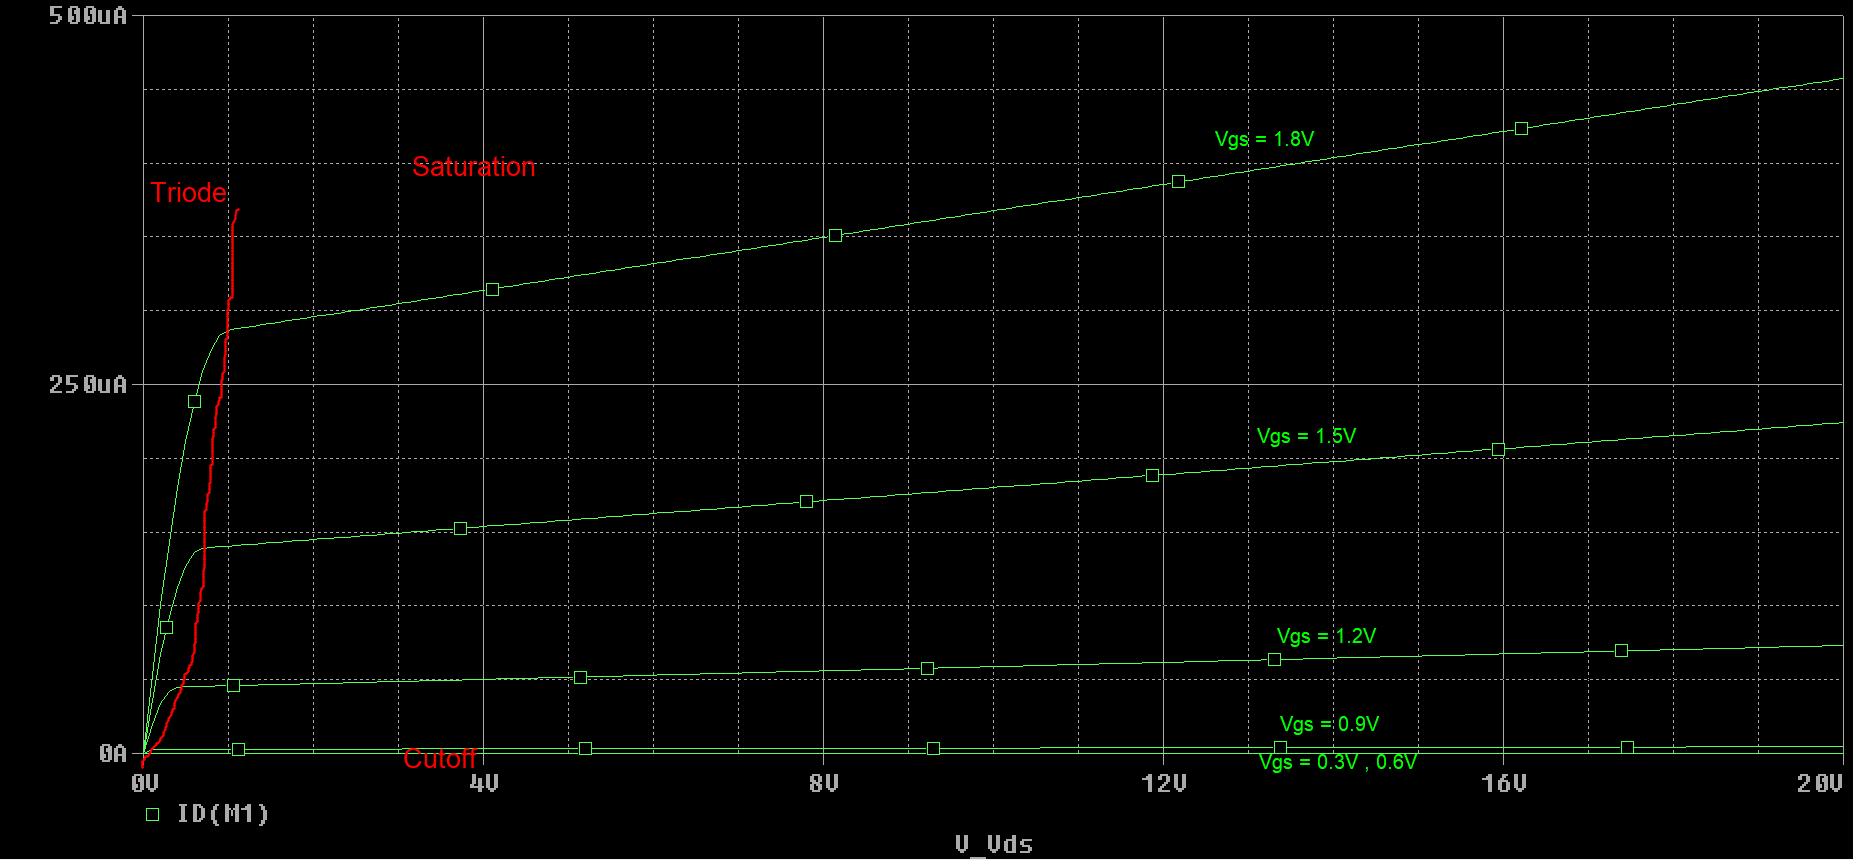
\includegraphics[scale=0.25]{./images/circuit1_vds_sweep.PNG}
	\caption{NMOS DC Sweep - $i_D$ vs $V_{DS}$}
	\label{fig:circuit1_vds_sweep}
\end{figure}

\FloatBarrier

\FloatBarrier

\begin{figure}[h!]
	\centering
	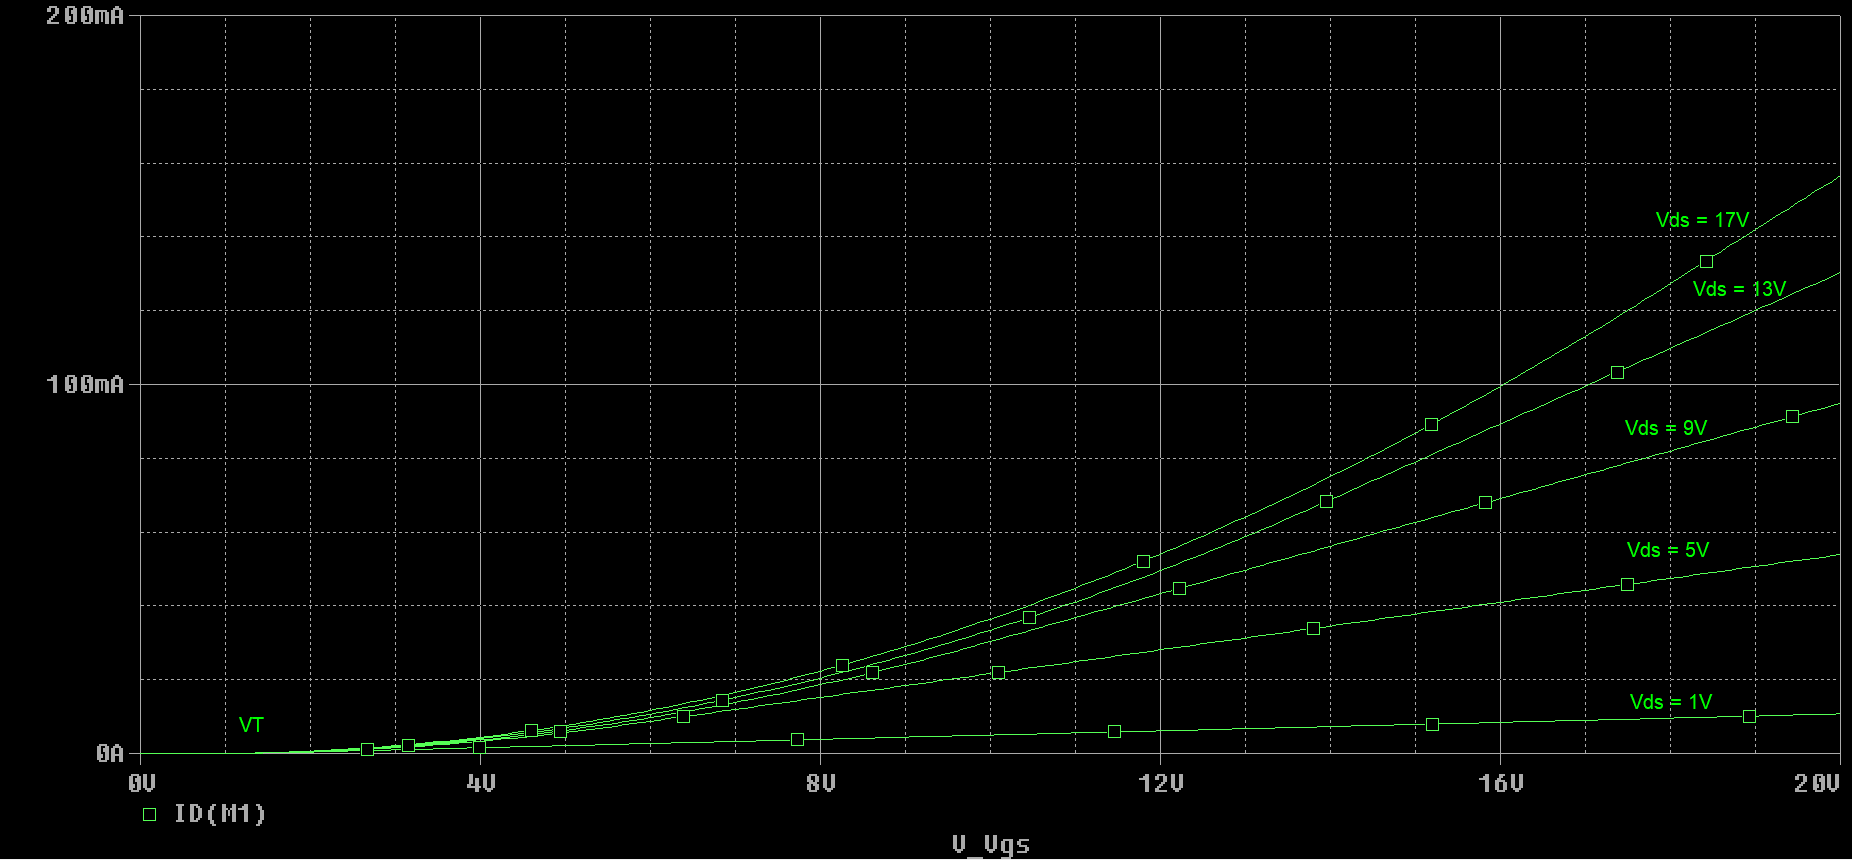
\includegraphics[scale=0.5]{./images/circuit1_full_sweep.PNG}
	\caption{NMOS DC Sweep - $i_D$ vs $V_{GS}$}
	\label{fig:circuit1_full_sweep}
\end{figure}

\FloatBarrier

When sweeping through increasing values of $V_{GS}$, the transistor goes from cutoff mode to saturation mode and eventually to triode mode. In the saturation mode, ignoring channel length modulation effects, the current varies approximately quadratically with $V_{GS}$:

\begin{equation}
	\label{eq:sat_current}
	i_D = \frac{k_n}{2} ( V_{GS} - V_{T} )^2
\end{equation}

Once $V_{GS}$ becomes sufficiently high, the transistor enters triode mode. At this point, the current has a linear dependence on $V_{GS}$:

\begin{equation}
	\label{eq:triode_current}
	i_D = k_n ( ( V_{GS} - V_{T} ) - \frac{V_{DS}}{2} ) V_{DS}
\end{equation}

So, the transistor should remain at zero, then grow quadratically, and then linearly. This is precisely the behavior observed in figure (\ref{fig:circuit1_full_sweep}). At higher $V_{DS}$ values, the transistor remains in saturation for longer due to the fact that $V_{DS} > V_{GS} - V_{T}$ remains true for more values of $V_{GS}$. So, the drain attains higher values before entering the linear triode region. As a result, the slope of the curve when in the triode region increases with $V_{DS}$. However, as $V_{DS}$ becomes large, the $i_D$ versus $V_{GS}$ curves asymptotically approach the curve $i_D = \frac{k_n}{2} ( V_{GS} - V_{T} )^2$ for all $V_{DS}$ values. When $V_{DS}$ is large, the transistor may not enter the triode region in this $V_{GS}$ range. This is why the curves begin to converge for larger $V_{DS}$ values. 
